In this approach, the precoders are designed iteratively by performing \ac{OTA} exchanges between the users and the coordinating \acp{BS} in the system. It is performed in the following approach. To begin with, let us assume that the initial transmit and the receive beamformers \me{\mvec{m}{l,k,n}^{(0)}}, \me{\mvec{w}{l,k,n}^{(0)}} are known to all the entities in the system. It is usually obtained by initial exchange of information about the local users receive beamformers through backhaul among the coordinating \acp{BS} \eqn{\mc{B}}. Once the initial receive equalizers are known at the transmitters, each \ac{BS} updates the transmit precoders for the \eqn{\ith{j}} exchange as
\begin{equation}
\mvec{m}{l,x,n}^{(j)} = \Big ( \sum_{k \in \mc{U}} \sum_{y=1}^L \alpha_{y,k,n}^{(j-1)} \mvec{H}{b_x,k,n}^\herm \mvec{w}{y,k,n}^{(j-1)} \mvec{w}{y,k,n}^{\herm \, {(j-1)}} \mvec{H}{b_x,k,n} + \delta_b \mbf{I}_{N_T} \Big )^{-1} \alpha^{(j-1)}_{l,x,n} \mvec{H}{b_x,x,n}^\herm \mvec{w}{l,x,n}^{(j-1)}
\end{equation}
Once the precoders are updated at each \ac{BS}, it is notified to all the users in the system through precoded downlink pilot \eqn{\mvec{H}{b_x,k} \mvec{m}{l,x,n}}, where \eqn{x \in \mc{U}_x} is the desired user and the precoder \eqn{\mvec{m}{l,k,n}} is notified to all the users in the system. 

Upon receiving the downlink precoded pilots, each user evaluate the equivalent downlink channel \me{\mvec{H}{b,k} \mvec{m}{l,x,n}} \eqn{\forall k\in \mathcal{U}} and use it to calculate the effective receive equalizers as
\begin{IEEEeqnarray}{RCL}
\mvec{w}{l,k,n}^{(j)} &=& \Big ( \sum_{x\in\mc{U}}\sum_{y=1}^L \mvec{H}{b_x,k,n} \mvec{m}{y,x,n}^{(j)} \mvec{m}{y,x,n}^{\herm \, (j)} \mvec{H}{b_{x},k,n}^\herm + \mathbf{I}_{N_R} \Big ) ^{-1} \; \mvec{H}{b_k,k,n} \; \mvec{m}{l,k,n}^{(j)} \\
\epsilon_{l,k,n}^{(j)} &=& \left | 1 - \mvec{w}{l,k,n}^{\herm \, (j)} \mvec{H}{b_k,k,n} \mvec{m}{l,k,n}^{(j)} \right |^2 + N_0 \, \|\mvec{w}{l,k,n}^{(j)}\|^2 + \sum_{\mathclap{(x,y) \neq (l,k)}} \left | \mvec{w}{l,k,n}^{\mathrm{H} \, (j)} \mvec{H}{b_y,k,n} \mvec{m}{x,y,n}^{(j)} \right |^2 \IEEEyessubnumber \label{kkt-mse-4.4} \\
t_{l,k,n}^{(j)} &=&  -\log_2(\epsilon_{l,k,n}^{(j-1)}) - \tfrac{\left ( \epsilon_{l,k,n}^{(j)} - \epsilon_{l,k,n}^{(j-1)} \right ) }{\log(2) \, \epsilon_{l,k,n}^{(j-1)}} \IEEEyessubnumber \label{kkt-mse-4.5} \\
\sigma_{l,k,n}^{(j)} &=& \Big [\tfrac{a_k \, q}{\log(2)}  \, \Big (Q_k - \sum_{n = 1}^N \sum_{l=1}^L t_{l,k,n}^{(j)} \Big )^{(q-1)}\Big ]^+  \IEEEyessubnumber \label{kkt-mse-4.2} \\
\alpha^{(j)}_{l,k,n} &=& \alpha^{(j-1)}_{l,k,n} + \rho \left ( \tfrac{\sigma_{l,k,n}^{(j)}}{\epsilon_{l,k,n}^{(j)}} - \alpha^{(j-1)}_{l,k,n} \right ) \IEEEyessubnumber \label{kkt-mse-4.1}
\end{IEEEeqnarray}
In order to notify the updated receivers, user will perform an uplink precoded pilot transmission, which is used to obtain the effective uplink channel at all \acp{BS} as \me{\sqrt{\alpha_{l,k,n}^{(j)}} \mvec{H}{b,k,n}^\tran \mvec{w}{l,k,n}^\ast} that will be used to evaluate the transmit beamformers for the next iteration \eqn{j+1}. In order to reduce the overhead, the number of \ac{OTA} exchanges required for the precoder convergence should be minimized. In the following sections, we discuss few approaches to achieve improved performance with limited number of signaling overhead.

\subsubsection{Centralized \ac{MSE}}
In this approach, the precoders are designed by a centralized controller, which knows the complete \ac{CSI} of all users in the system and the precoders are iterated until convergence. It is used as benchmark in the distributed precoder design procedures.

\subsubsection{\ac{MSE} with }



\begin{figure*}
	\centering
	\subfloat[][Average Transmitted Packets after each of \me{500} transmission instants]{
		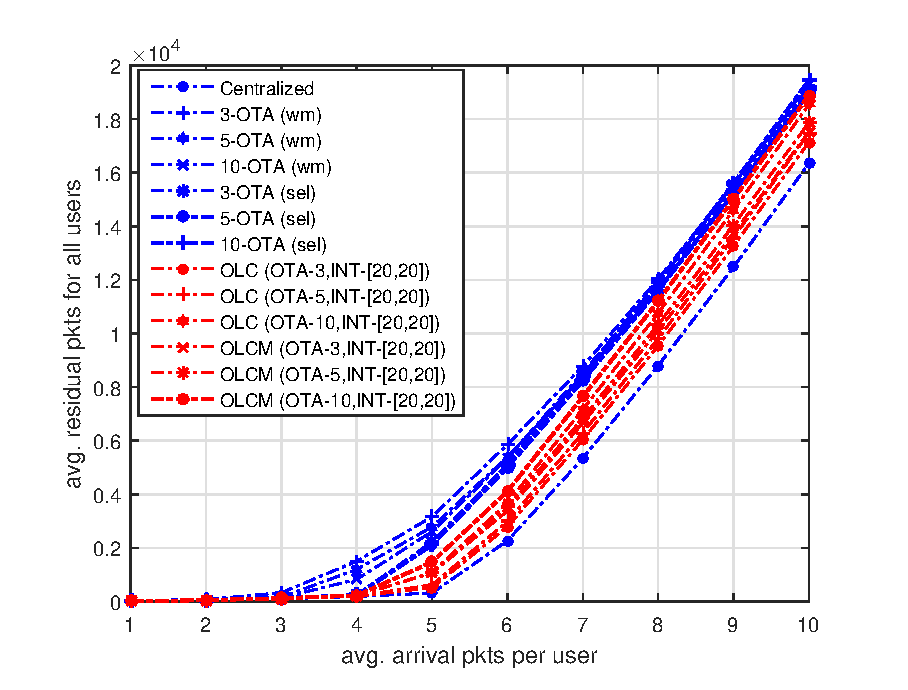
\includegraphics[width=0.48\textwidth]{fig-1}
		\label{fig-review}
	}
	\hfill
	\subfloat[][Average Residual packets after each of \me{500} transmission instants]{
		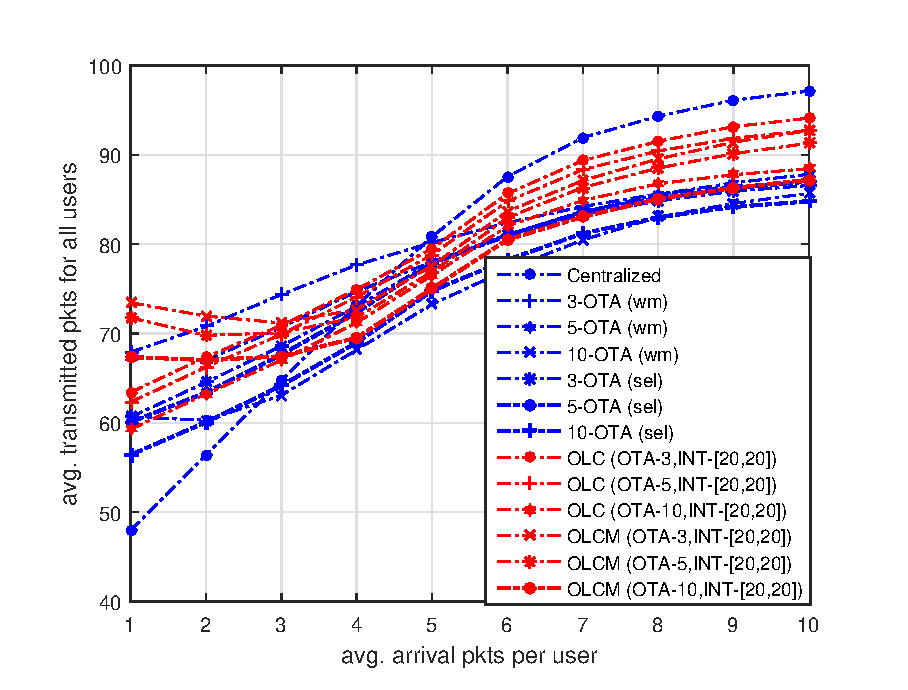
\includegraphics[width=0.48\textwidth]{fig-2}
		\label{fig-review-time}
	}
	\caption{Queue dynamics for a system \me{\lbrace N,N_B,K,N_T,N_R \rbrace = \lbrace 4,2,16,4,2 \rbrace}}
	\label{fig-time-analysis}
\end{figure*}


\begin{figure*}
	\centering
	\subfloat[][Average Transmitted Packets after each of \me{500} transmission instants]{
		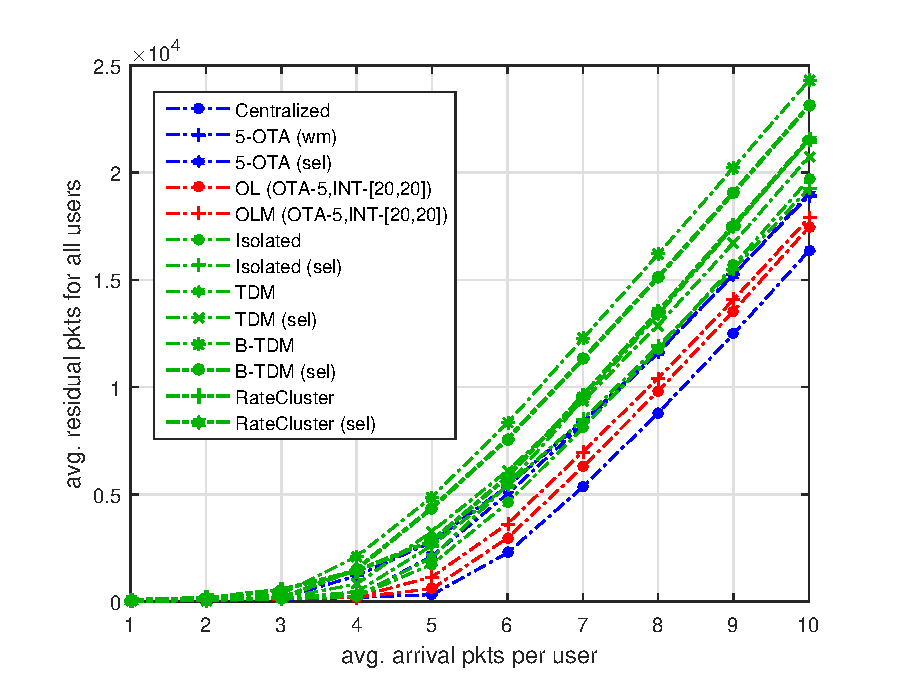
\includegraphics[width=0.48\textwidth]{fig-3}
		\label{fig-review}
	}
	\hfill
	\subfloat[][Average Residual packets after each of \me{500} transmission instants]{
		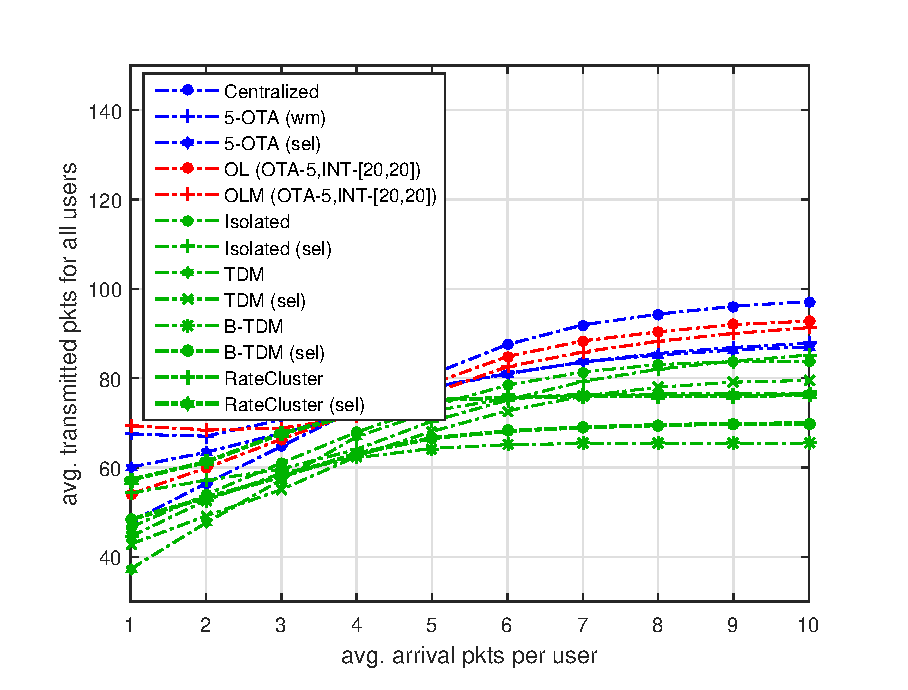
\includegraphics[width=0.48\textwidth]{fig-4}
		\label{fig-review-time}
	}
	\caption{Queue dynamics for a system \me{\lbrace N,N_B,K,N_T,N_R \rbrace = \lbrace 4,2,16,4,2 \rbrace}}
	\label{fig-time-analysis}
\end{figure*}

